\section{Demystify Microarchitecture Features}
\label{sec:assembler}

\subsection{Methodology}
We propose a methodology to demystify GPU microarchitecture features and correlate them with performance. The workflow consists of three components: CUDA binary tools, a instruction solver, and a rigorous microbhenchmark. We leverage CUDA binary tools to generate assembly codes for sample programs or libraries. A sample program is a synthetic CUDA file targeted to generate some specific instructions. A library might provide a high coverage of instruction sets. For example, the CUBLAS library contains almost all instructions used in SGEMM routines. As introduced in section~\ref{sec:cuda}, these generated assembly files ({\em sass}) provide a instruction encoded number to be cracked.

The instruction solver takes the assembly files as input to decode 64-bits binary representation of each instruction. We design a set of algorithms to solve all fields of the binary instruction. These fields include {\em register, predicate, address, immediate, constant} and {\em opcode}. The solver retrieves the undocumented ISA specification, which is used to implement an native assembler. Then, we design a rigorous microbenchmark and leverage the assembler to tune code at assembly language level. In the end, the tuning process will lead to some practical observations on the correlation between microarchitecture and performance.

\begin{figure}[htbp]
\begin{center}
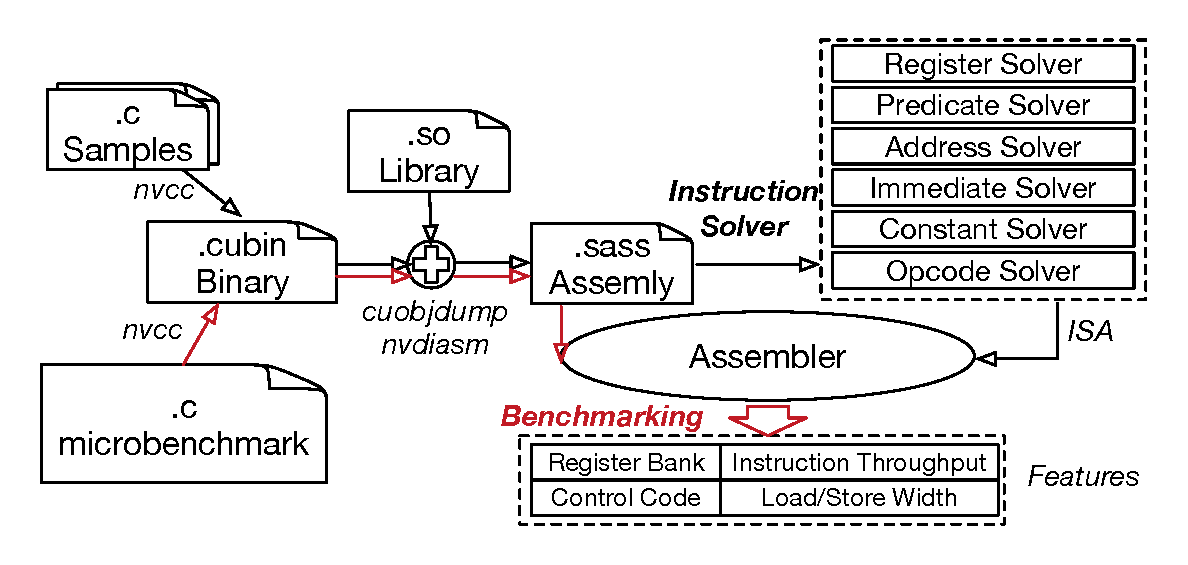
\includegraphics[scale=0.45]{methodology}
\caption{A schematic diagram of demystifying GPU microarchitecture features by leveraging CUDA binary tools. The back arrows represent the workflow of instruction solver while the red ones represents that of benchmarking to find out correlation between microarchitecture and performance.}
\label{fig:workflow}
\end{center}
\end{figure}

\subsection{Instruction Solver}
An instruction is composed of three fields: {\tt opcode}, {\tt operands} and {\tt modifiers}. An operand can be register, constant memory, global memory, shared memory, immediate, or predicate register.
The encoding of operands can be inferred by their names. For instance, the register operand {\tt R5} could be
inferred as $101$ in binary format, immediate $0x9$ is represented as $1001$. Besides, the fixed lengths of these fields allow us to determine their positions and lengths and hence encoding. Encodings of opcode and modifier are mnemonic symbols, we can not infer encoding by their names. Modifiers are instruction specific, the same kind of modifier can be different encodings for different instructions. For instance, mask of type-size
modifier for {\tt LD} and {\tt LDG} are at different positions. So we deal with modifier for each instruction separately.

\subsubsection{Operands:Fixed Length Field}

The basic idea of Algorithm~\ref{algo:int_solver} is that match binary encoding of operand in $64$ instruction encoding and find
position until the postion is unique. The input instructions are from disassembly code (i.e., NVIDIA CUBLAS library).
First, we randomly pick up instruction that has the filed we want to probe, and represent it in binary by its name. Second, we match its binary in $64$-bit instruction encoding, and find possible positions. Third, we intersect current candidate with previous one, if the number of candidate is $1$, we find the position. Otherwise, we set the current candidate to the previous one and randomly pick next instruction to repeat the procedure.

\begin{algorithm}
      \caption{Solver}
      \label{algo:int_solver}
  \begin{algorithmic}[1]
	  \State \textbf{input:} instmap
      \State output: pos, length
      \State currpos=\{\}
      \State prepos=\{0,1,2,...63\}
      \While {lenght(currpos) != 1}
      \State inst=instmap[random()]
      \If {inst.src1type == immediate}
      \State instencode=inst->encode64bit
      \State immbin = completecode(imm)
      \State pos = 0
      \While {pos + length(immbin) < 64}
      \If {strcmp(immbin,instencode+pos,length(immbin)}
      \State pushback(currpos, pos)
      \EndIf
      \EndWhile
      \State currpos = intersect (curpos, prepos)
      \State prepos = currpos
      \State currpos=\{\}
      \EndIf
      \EndWhile
      \State return curpos[0]
  \end{algorithmic}
\end{algorithm}


After finding the operand position, we need to infer or veritify the length of operand encoding. Some are easy to be
inferred, for example, there are at most $256=2^{8}$ registers for each thread, we could infer the length of register operand to be $8$.
The others like immediate or script note of constant memory is more complicated. One solution is to set the bit from the
position one by one to check whether the operand value is grown as we expected.

\subsubsection{Opcode}
Opcodes does not show their encoding literally. One possible way is to write instruction {\tt PTX} code with flags
combinations based on syntax on NVIDIA PTX manual, and generate encoding by using NVDIA toolchain.
Then, opcode can be got by stripping out operand mask, and flags can be found by stripping out opcode and operand mask. However, the uncompleteness of NVIDIA document hinder us to find out all the opcodes and instruction modifiers. Another feasible way is to emulate all of possible binary combinations after striping out operand mask.
Normally, each instruction have $3$ register operand, and one $4-bit$ predicate register, we have $64-8*3-4=36$ bits left to probe.
In fact, we can further prune the search space by recognizing possible position by algorithm~\ref{algo:opcode}. By randomly probing bit by bit, we find that the top $10$ bits and lower $2$ bits represent opcode and other bits represent flags. Thus, we only enumerate these opcode bits which generate a acceptable search space. Finally, we find the minimal opcode without any flags. 


\begin{algorithm}
      \caption{Opcode Solver}\label{algo:opcode}
  \begin{algorithmic}[1]
      \State for each instruction in PTX generated database
      \For {i=0; i < num\_inst; i++}
      \For {j=0; j < 64; j ++}
      \If {isoperand(encode[i][j] == 0) and encode[i][j]== 0}
      \State newcode = encode[i][j].setbit(j, 1)
      \State newinst=nvdisasm(newcode)
      \If {sameop(newinst,oldinst) == 0 and isvalid(newinst) }
      \State pushback(j)
      \EndIf
      \EndIf
      \EndFor
      \EndFor
  \end{algorithmic}
\end{algorithm}

\subsubsection{Modifier: Instruction Specific}

Modifier defines a specific behavior for some instruction. For example,
{\tt LD} instruction has type-size modifiers, such as .u8, .s8, .u16, .32, .64 and .128. {\tt LD} also has cache operation modifier, such as .ca(cache at all level) and .cg(cache at global level). Modifiers (also called flags) are much more complicated because its position spans accross the reminding bits and one instruction may have more than one kinds of modifiers. By excluding both opcode and operand mask, there remain around $24$ bits. We observe that the default value for modifier is $0$. That is, modifier works when at least one bit is set. We can find possible positions of modifiers 
by greedily set the remaining bits one by one, the time complexity is $O(2^{10})$ instead of $O(2^{24})$. The number of bit is typically less
than $10$. After finding the candidates, we enumerate these bits, and group each kind.

\subsection{Correlating Microarchitecture with Performance}
With the assembler we tune the assembly codes of microbenchmark. According to the performance tuning results, we correlate microarchitecture with performance variants that guide performance optimizations in real applications. The correlation is presented as several meaningful observations, which are categorized into four microarchitectural features of {\tt control} function, {\tt register} allocation, {\tt arithmetic} throughput and {\tt memory} operation.

\begin{figure}[htbp]
\begin{center}
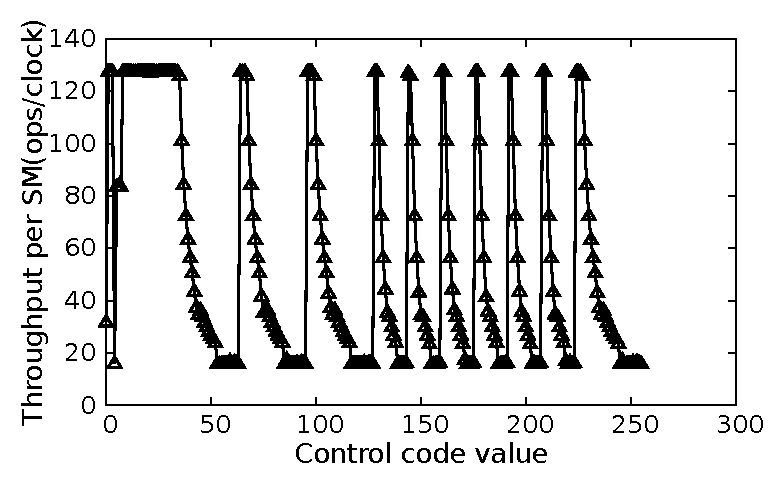
\includegraphics[scale=0.5]{ctrl}
\caption{Different control codes regulate {\tt FFMA} throughput.}
\label{fig:control_throughput}
\end{center}
\end{figure}

\begin{figure}[htbp]
\begin{center}
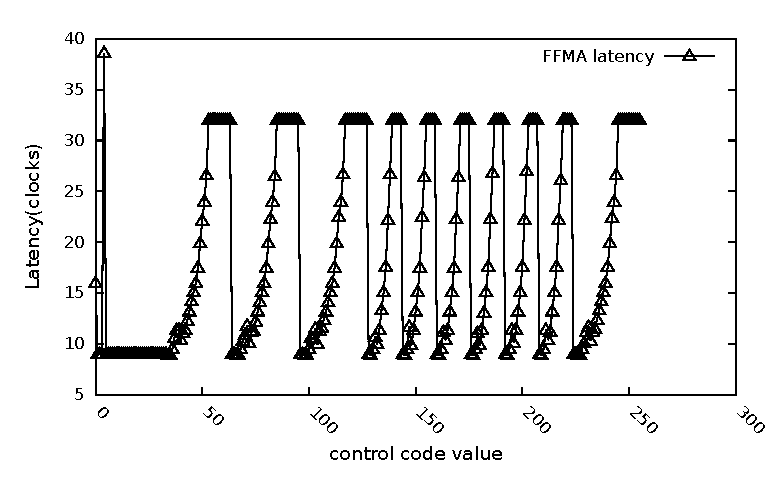
\includegraphics[scale=0.5]{ctrl_latency}
\caption{Different control codes regulate {\tt FFMA} latency.}
\label{fig:control_latency}
\end{center}
\end{figure}

\begin{figure}[htbp]
\begin{center}
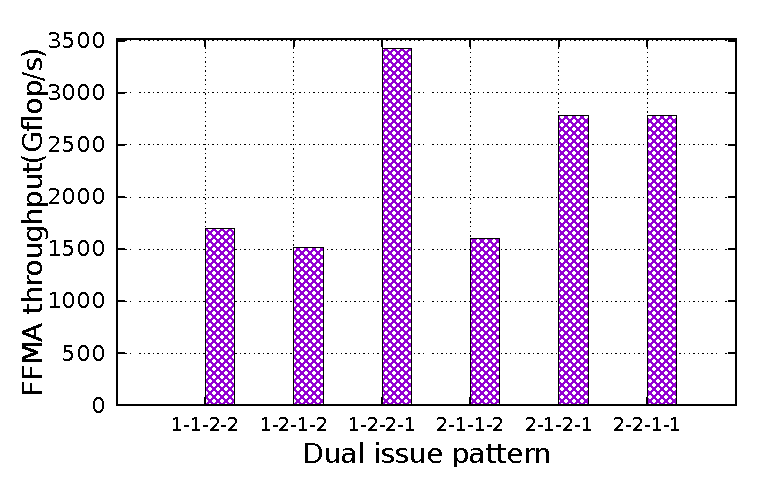
\includegraphics[scale=0.5]{pattern}
    \caption{Control codes pattern regulate peak {\tt FFMA} throughput(S:single issue, D:dual issue).}
\label{fig:pattern}
\end{center}
\end{figure}

{\em {\bf Observation 1--[Control]}: The execution sequence of instructions is regulated by control codes. Both warp scheduling and issue mode are tunable by setting control codes.}

Starting with the Kepler architecture NVIDIA has been moving some control logic off of the chip and into kernel instructions which are determined by the assembler. This evolution provides programmer a chance to make globally optimal decisions on scheduling and other control aspects if an assembler is available. The disassembly code indicates that every 64 bits control code controls $7$ instructions. We identify that both higher $6$ bits and lower 2 bits are {\em opcode} of control code, and the middle 56 bits are used to control the execution of $7$ instructions, each of which is assigned $8$ control bits.

For the eight control bits, we identify their meanings by examining CUBLAS disassembly codes and tuning a {\tt FFMA}
throughput microbhenchmark. We observe that the $7$th bit of the control code of {\tt TLD} instruction is $1$, which
indicates a texture dependency barrier due to weak consistent memory model. It's verified that some illegal values are
loaded if this bit is not set. Similarly, we discover that the $5$th bit means shared memory dependency barrier, the
$4$th bit means global memory dependency barrier. Figure~\ref{fig:control_throughput} shows that {\tt FFMA} throughput varies with all control bit values from 0 to 255. As shown in this figure, the throughput linearly decreases with the increasing values represented by the $0-3$ bits. That implies that these $4$ bits set the number of stall cycles before issuing the instruction. Further, the microbenchmarking reveal some specific patterns of control codes:

\begin{itemize}
\item When the control bits are set to be $0x40$, the scheduler suspends a warp of the instructions for 32 cycles.
\item $0x04$ means dual issue mode. If two consecutive instructions is controlled by $0x04$ and $0x05$, the throughput can reach the maximum. Single issue control code is $0x00$.
\item $0x20|n$ means a warp is suspended for $n$ cycles before issuing the next instruction, where $n$ is number between 0 and 15.
\end{itemize}


{\em {\bf Observation 2--[Register]}: Irrespective of single- or dual-issue mode, register bank conflict is only caused by source operands, and degrades instruction throughput by up to $17\%$.}

For CUDA programming model it is well-known that shared memory bank conflict is an important performance factor. In
fact, recent researches~\cite{lai} noticed that register bank conflicts are nontrivial to performance.  In order to probe register bank conflict, our microbenchmark measures instruction throughput for different combination of {\tt FFMA} register operands. Table~\ref{tab:th} shows an example of the combination which results in variance of efficiency. The numbers in the fifth column represent the number of registers conflict in the same bank. This experiment is conducted in single-issue mode by setting control code to be $0x20$. The theoretical efficiency is $128/192=66.67\%$. In fact, we observe that both single- and dual-issue mode produce the same variance of instruction throughput. Besides, from the experimental results we observe that:
\begin{itemize}
\item Destination operand will not contribute to bank conflict, no matter which bank is assigned to it.
\item When source operands have 2-way conflict, the throughput will drop by 2.33\% in single issue
    mode. When source operands have 3-way conflicts, the throughput will drop by 17.17\%.

 \item On Kepler architecture, our microbenchmark finds out a proper distribution of registers for eliminating bank
     conflict. The distribution is summarized in Table~\ref{tab:reg}, which confirms the follow the rule~\cite{lai}: \\
 bank0$\Leftarrow$($Rindex \% 8 < 4$ \&\& $Rindex \% 2 == 0$) \\
 bank2$\Leftarrow$($Rindex \% 8 < 4$ \&\&
$Rindex \% 2 == 1$) \\
bank1$\Leftarrow$($Rindex \% 8 > 4$ \&\& $Rindex \%2 == 0$) \\
bank3$\Leftarrow$($Rindex \% 8 < 4$ \&\&
$Rindex\% 2 == 1$)\\
where $Rindex$ is the register number. This rule will guide the performance tuning in the following SGEMM implementation.

\end{itemize}

\begin{table}[htbp]
\caption{The efficiency of instruction throughput varies with difference register bank distribution. {\it Inst} : instruction pattern, {\it Th/SM}: the instruction throughput per SM, {\it Eff}: efficiency of throughput.}
\centering
\scalebox{1.0} {
\begin{tabular}{|c||c|c|c|}
\hline
Inst &Th/SM&Eff&Conflicts \\
\hline
{\tt FFMA R5,R4,R1,R0}&127.50&66.40\%&0\\
\hline
{\tt FFMA R2,R4,R1,R0}&127.50&66.40\%&0\\
\hline
{\tt FFMA R5,R2,R1,R0}&119.18&62.07\%&2\\
\hline
{\tt FFMA R3,R2,R1,R0}&119.18&62.07\%&2\\
\hline
{\tt FFMA R5,R9,R3,R1}&94.52&49.23\%&3\\
\hline
{\tt FFMA R11,R9,R3,R1}&94.52&49.23\%&3\\
\hline
{\tt FMUL R4,R1,R0}&127.50&66.40\%&0\\
\hline
{\tt FMUL R4,R2,R0}&119.17&62.06\%&2\\
\hline
\end{tabular}
}
\label{tab:th}
\end{table}


\begin{table}[htbp]
\caption{Register distribution for zero bank conflict.}
\centering
\scalebox{1.0} {
\begin{tabular}{|c||c|c|c|c|c|c|c|c|c|}
\hline
Bank0&0&2&8&10&16&18&24&26&... \\
\hline
Bank1&1&3&9&11&17&19&25&27&... \\
\hline
Bank2&4&6&12&14&20&22&28&30&... \\
\hline
Bank3&5&7&13&15&21&23&29&31&...\\
\hline
\end{tabular}
}
\label{tab:reg}
\end{table}

{\em {\bf Observation 3--[Arithmetic]}: With a proper control code and register allocation, {\tt FFMA} instruction throughput can approach the theoretical peak in dual issue mode.}

It's very intricate to tune instruction execution to improve instruction throughput. The previous work report a maximal throughput of {\tt FFMA} on a SM is $132$, which is much less than the theoretical throughput $192$ on Kepler. Our microbenchmarks reveal several key points of optimization to approach theoretical peak on Kepler. First, the control code must be set properly to dual issue adjacent instructions. Second, the ratio and interval of dual issue {\tt FFMA} instructions must be tuned into a specific pattern. Since each warp of extra computing unit is shared among two warps, when all threads are trying to fully dual issue every two adjacent {\tt FFMA}s, half of the scheduler would stall due to computing resource conflict. The ratio of dual issue and single issue should be $2:2$, and with a proper phase shift among two warp's executing pace, they could get access to the shared computing unit in turn. Third, the first instruction of the core loop needs to be aligned. This restriction is caused by the aligned position of control code in the instruction sequence. Last, {\tt FFMA} dual issue requires 6 register banks. Instruction order has to be adjusted to fully use Kepler's operand collector mechanism to avoid register bank conflicts. As shown in Table~\ref{tab:ffma}, these optimizations together improve {\tt FFMA}'s throughput  to be $190$, which is very close to the theoretical peak $192$.

\begin{table}[htbp]
\caption{Floating-point instruction throughput on Kepler}
\centering
\scalebox{1.} {
\begin{tabular}{|c||c|c|c|}
\hline
Inst name&operation&single issue&dual issue\\
\hline
{\tt FFMA} &c=a*b+c&127.52&190.35 \\
\hline
{\tt FMUL} &c=a*b&127.52&190.35 \\
\hline
{\tt FADD} &c=a+b&127.52&192\\
\hline
\end{tabular}
}
\label{tab:ffma}
\end{table}


{\em {\bf Observation 4--[Memory]}: For achieving higher memory bandwidth, shared memory prefers to 64-bits load instruction {\tt LDS.64} while global memory prefers to 128-bits load instruction {\tt LDG.E.128} with texture path.}

For the GPU memory hierarchy we focus on the programmer controllable memory resources--shared memory and global memory. On NVIDIA GPU architecture, there are different memory access widths (i.e., 32-bits,64-bits,128-bits) and paths (i.e., normal cache or texture cache). In fact, both NVIDIA document and previous works~\cite{} pointed out that wider instructions have longer pipeline latencies, which are also measured in our microbenchmark. In addition, we identify several bandwidth issues for memory optimization.

Intuitively, a wider load operation achieves higher bandwidth. We benchmark bandwidth of shared memory operations {\tt LDS} with different widths, i.e., {\tt LDS.32}, {\tt LDS.64}
and {\tt LDS.128}. The operations are specially arranged so that no shared memory bank conflict occurs in a warp. In the
experiment, the amount of data are projected to the number of load instructions. For exmaple, if the data are loaded by
$N$ {\tt LDS.128} instructions, then either $2N$ {\tt LDS.64} or $2N$ {\tt LDS.64} instructions are required.
Figure~\ref{fig:lds_bw} compares the sequential memory access bandwidth with increasing volume of data. As shown in the figure, {\tt LDS.64} achieves the highest bandwidth $113GB/s$, which is about $60\%$ of the peak bandwidth\footnote{The theoretical shared memory bandwidth for each SM can be calculated as $Bandwidth=f_{core}*Width*Warpsize$ in
bytes, where $f_{core}$ is frequency of CUDA core, $Width$ is bank width, $Warpsize$ is warp size.}.

\begin{figure}[htbp]
\begin{center}
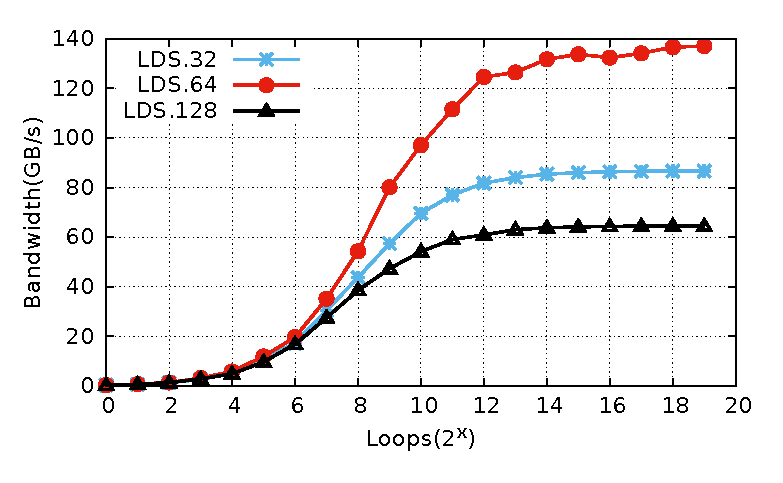
\includegraphics[scale=0.6]{lds_bandwidth}
    \caption{ Bandwidth of {\tt LDS.32}, {\tt LDS.64} and {\tt LDS.128}}
\label{fig:lds_bw}
\end{center}
\end{figure}

% global memory
There are two paths to global memory. One is from global memory to normal cache (L1 or L2), which is executed by {\tt
LD} instruction. The other one is from global memory to texture cache, which is executed by {\tt LDG} instruction. We
launche $26$ thread blocks with $512$ threads, and specifies that each thread access $4$ words with a stride of
$4*blockDim.x*gridDim.x$. Our benchmark confirms that {\tt LDG} achieves higher bandwidth than {\tt LD}, which has been
identified by previous work~\cite{tan}.
